\documentclass{article}
\usepackage[top=1in, bottom=1in, left=1in, right=1in]{geometry}
\usepackage{graphicx}
\begin{document}

\begin{flushright}
Matt Jibson \\
EG 510 \\
HW 11
\end{flushright}

\begin{enumerate}
	\item
		\begin{itemize}
			\item [(a)] Graphical solution: $x_1 = 0, x_2 = 4, -x_1 - x_2 = -4$: \\
				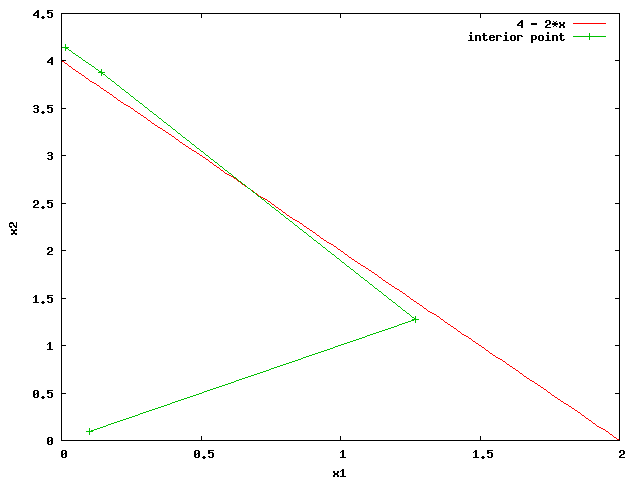
\includegraphics[width=0.8\linewidth]{1a.png}
			\item [(b)]
				\begin{displaymath}
					\mathbf{x}_0 = \left[ \begin{array}{c} 0.1 \\ 0.1 \\ 3.9 \end{array} \right],
					\mathbf{D} = \left[ \begin{array}{c c c} 0.1 & 0 & 0 \\ 0 & 0.1 & 0 \\ 0 & 0 & 3.9 \end{array} \right],
					\mathbf{B} = \mathbf{AD} = \left[ \begin{array}{c c c} 0.2 & 0.1 & 3.9 \end{array} \right],
				\end{displaymath}
				\begin{displaymath}
					\mathbf{BB}^T = \left[ \begin{array}{c} 15.26 \end{array} \right], \mathbf{Dc} = \left[ \begin{array}{c c c} -0.1 \\ -0.1 \\ 0 \end{array} \right], \mathbf{BDc} = \left[ \begin{array}{c} -0.03 \end{array} \right],
				\end{displaymath}
				\begin{displaymath}
					\mathbf{w} = \left[ \begin{array}{c} -0.001966 \end{array} \right], \mathbf{c}_p = \left[ \begin{array}{r} 0.0996 \\ 0.0998 \\ -0.007667 \end{array} \right], \theta = 1/0.007667 = 130.43, \alpha = 0.9 \Rightarrow
				\end{displaymath}

				\begin{displaymath}
					\mathbf{x}_1 = \left[ \begin{array}{c} 1.269 \\ 1.272 \\ 0.39 \end{array} \right],
					\mathbf{D} = \left[ \begin{array}{c c c} 1.269 & 0 & 0 \\ 0 & 1.272 & 0 \\ 0 & 0 & 0.39 \end{array} \right],
					\mathbf{B} = \mathbf{AD} = \left[ \begin{array}{c c c} 2.538 & 1.272 & 0.39 \end{array} \right],
				\end{displaymath}
				\begin{displaymath}
					\mathbf{BB}^T = \left[ \begin{array}{c} 8.212 \end{array} \right], \mathbf{Dc} = \left[ \begin{array}{c c c} -1.269 \\ -1.272 \\ 0 \end{array} \right], \mathbf{BDc} = \left[ \begin{array}{c} -4.839 \end{array} \right],
				\end{displaymath}
				\begin{displaymath}
					\mathbf{w} = \left[ \begin{array}{c} -0.5893 \end{array} \right], \mathbf{c}_p = \left[ \begin{array}{r} -0.2265 \\ 0.5225 \\ -0.2298 \end{array} \right], \theta = 1/0.2298 = 4.352, \alpha = 0.9 \Rightarrow
				\end{displaymath}

				\begin{displaymath}
					\mathbf{x}_2 = \left[ \begin{array}{c} 0.1433 \\ 3.875 \\ 0.039 \end{array} \right],
					\mathbf{D} = \left[ \begin{array}{c c c} 0.1433 & 0 & 0 \\ 0 & 3.875 & 0 \\ 0 & 0 & 0.039 \end{array} \right],
					\mathbf{B} = \mathbf{AD} = \left[ \begin{array}{c c c} 0.2866 & 3.875 & 0.039 \end{array} \right],
				\end{displaymath}
				\begin{displaymath}
					\mathbf{BB}^T = \left[ \begin{array}{c} 15.1 \end{array} \right], \mathbf{Dc} = \left[ \begin{array}{c c c} -0.1433 \\ -3.875 \\ 0 \end{array} \right], \mathbf{BDc} = \left[ \begin{array}{c} -15.0567 \end{array} \right],
				\end{displaymath}
				\begin{displaymath}
					\mathbf{w} = \left[ \begin{array}{c} -0.9972 \end{array} \right], \mathbf{c}_p = \left[ \begin{array}{r} -0.1425 \\ 0.011 \\ -0.03889 \end{array} \right], \theta = 1/0.1425 = 7.018, \alpha = 0.9 \Rightarrow
				\end{displaymath}

				\begin{displaymath}
					\mathbf{x}_3 = \left[ \begin{array}{c} 0.0143 \\ 4.143 \\ 0.0294 \end{array} \right]
				\end{displaymath}

				On the graph the interior point method is clearly infeasible. Is this due to a calculation or procedure error on my part? Or is it just rounding and sig fig stuff?

			\item [(d)] Dual is: \\
				\begin{displaymath}
					\begin{array}{ll}
					\textrm{maximize} & w = 4y_1 \\
					\textrm{subject to} & 2y_1 \ge -1 \\
					& y_1 \ge -1 \\
					& y_1 \le 0
					\end{array}
				\end{displaymath}

				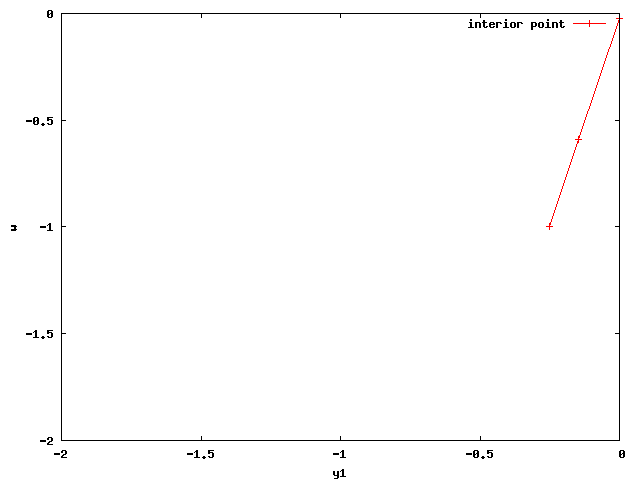
\includegraphics[width=0.7\linewidth]{1d.png}

				Here we see the feasible range is $-0.5 \le y_1 \le 0$, and the \textbf{w}'s generated in the affine scaling alrorithm are converging on the dual solution.

		\end{itemize}
\end{enumerate}

\end{document}
